\section{Introduction}

\subsection{Purpose}
This document presents a detailed description of the web application a-bec.
First and foremost, it provides a legally binding contract between the
stakeholders and the developer team 9. This document is a RUP conform SRS document.

\subsection{Scope of the Project}
The web application Flatfindr will help the participating user to promote or
find vacant places.

More specifically, the application will provide methods to search for vacant
flats, help to ensure flats with specific parameters are presented for users and
that the application will provide enough methods to get in contact with the
advertiser. On the other hand, users will be able to insert an ad for a vacant
place, will help define the visitation time (if a user wants to
see the flat which is advertised) and provide some other instruments to describe
the flat as best as possible.

\subsection{Glossary}

\begin{table}[H]
	\centering
	\begin{tabular}{p{3cm}p{9cm}}
	\multicolumn{1}{c}{\textbf{Term}} & \multicolumn{1}{c}{\textbf{Description}} \\
Advertiser & User who advertises his vacant place. \\
RUP & Stands for Rational Unified Process. Process developed by IBM. Has the SRS document as a requirement for all development activities. \\
SRS & Stands for Software Requirements Specification. A document that completely describes all of the functions of a proposed system and the constraints under which it must operate. \\
Stakeholder & Any person with an interest in the project who is not a developer. \\
User & Participant in the application. Can either be a normal user who searches
for a place or an advertiser.
	\end{tabular}
	\caption{Glossary}
	\label{table-glossary}
\end{table}

\subsection{Stakeholders}
Table \ref{table-stakeholders} will give an overview of the known
Stakeholders.
\begin{table}[H]
	\centering
	\begin{tabular}{ll}
	\multicolumn{1}{c}{\textbf{Name}} & \multicolumn{1}{c}{\textbf{Contact}} \\
	Haidar Osman & haidaros on GitHub                                        
	\end{tabular}
	\caption{Stakeholders}
	\label{table-stakeholders}
\end{table}

\subsection{System Overview}
Image \ref{image-system-overview} will introduce a general system overview
of the product in development.
\begin{figure}[p]
    \centering
	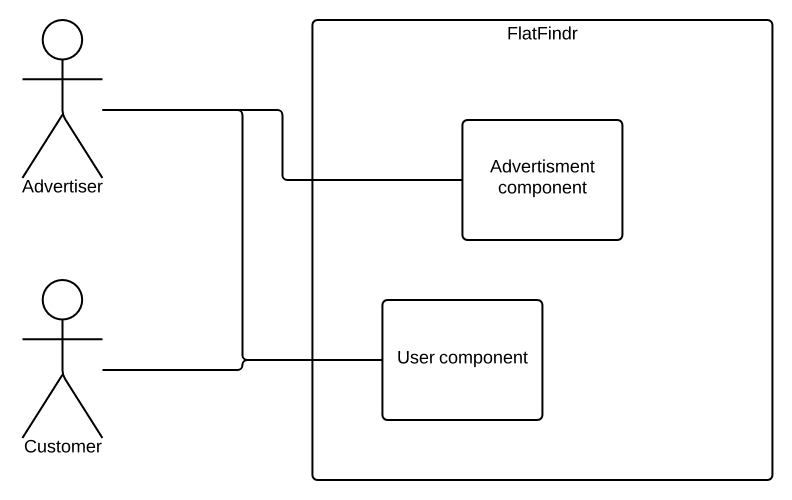
\includegraphics[width=12cm]{images/system-overview}
	\caption{System Overview}
    \label{image-system-overview}
\end{figure}

\subsection{References}
